% Options for packages loaded elsewhere
\PassOptionsToPackage{unicode}{hyperref}
\PassOptionsToPackage{hyphens}{url}
%
\documentclass[
]{article}
\usepackage{amsmath,amssymb}
\usepackage{lmodern}
\usepackage{ifxetex,ifluatex}
\ifnum 0\ifxetex 1\fi\ifluatex 1\fi=0 % if pdftex
  \usepackage[T1]{fontenc}
  \usepackage[utf8]{inputenc}
  \usepackage{textcomp} % provide euro and other symbols
\else % if luatex or xetex
  \usepackage{unicode-math}
  \defaultfontfeatures{Scale=MatchLowercase}
  \defaultfontfeatures[\rmfamily]{Ligatures=TeX,Scale=1}
\fi
% Use upquote if available, for straight quotes in verbatim environments
\IfFileExists{upquote.sty}{\usepackage{upquote}}{}
\IfFileExists{microtype.sty}{% use microtype if available
  \usepackage[]{microtype}
  \UseMicrotypeSet[protrusion]{basicmath} % disable protrusion for tt fonts
}{}
\makeatletter
\@ifundefined{KOMAClassName}{% if non-KOMA class
  \IfFileExists{parskip.sty}{%
    \usepackage{parskip}
  }{% else
    \setlength{\parindent}{0pt}
    \setlength{\parskip}{6pt plus 2pt minus 1pt}}
}{% if KOMA class
  \KOMAoptions{parskip=half}}
\makeatother
\usepackage{xcolor}
\IfFileExists{xurl.sty}{\usepackage{xurl}}{} % add URL line breaks if available
\IfFileExists{bookmark.sty}{\usepackage{bookmark}}{\usepackage{hyperref}}
\hypersetup{
  pdftitle={Methodological Details - Blue Bananas},
  hidelinks,
  pdfcreator={LaTeX via pandoc}}
\urlstyle{same} % disable monospaced font for URLs
\usepackage[margin=1in]{geometry}
\usepackage{graphicx}
\makeatletter
\def\maxwidth{\ifdim\Gin@nat@width>\linewidth\linewidth\else\Gin@nat@width\fi}
\def\maxheight{\ifdim\Gin@nat@height>\textheight\textheight\else\Gin@nat@height\fi}
\makeatother
% Scale images if necessary, so that they will not overflow the page
% margins by default, and it is still possible to overwrite the defaults
% using explicit options in \includegraphics[width, height, ...]{}
\setkeys{Gin}{width=\maxwidth,height=\maxheight,keepaspectratio}
% Set default figure placement to htbp
\makeatletter
\def\fps@figure{htbp}
\makeatother
\setlength{\emergencystretch}{3em} % prevent overfull lines
\providecommand{\tightlist}{%
  \setlength{\itemsep}{0pt}\setlength{\parskip}{0pt}}
\setcounter{secnumdepth}{5}
\usepackage{expex}
\lingset{everygla=,everyglpreamble=\it}
\ifluatex
  \usepackage{selnolig}  % disable illegal ligatures
\fi

\title{Methodological Details - Blue Bananas}
\author{}
\date{\vspace{-2.5em}9/17/2020}

\begin{document}
\maketitle

\hypertarget{research-questions}{%
\section{Research Questions}\label{research-questions}}

This study investigates whether speakers modify the speech signal to
signal atypical referents? Concretely, we ask whether the suprasegmental
profile of an utterance with an atypical referent like ``blue banana''
is different from one with a typical referent such as ``yellow banana''.

\hypertarget{participants}{%
\section{Participants}\label{participants}}

Thirty native German speakers participated in this study. All
participants grew up in a monolingual environment and were recruited
from the population living in the broad Cologne area with normal or
corrected-to-normal vision and normal hearing. Participants were paid
for their participation.

\hypertarget{procedure}{%
\section{Procedure}\label{procedure}}

In this production study, participants interacted with the experimenter.
Participants had to verbally instruct the experimenter to select a
specified target object out of four visually presented objects. The
non-target objects differed from the target with respect to their
colour, their identity, or both. Objects were referred to using noun
phrases that consist of a modifier denoting colour and a modified object
(e.g.~yellow banana, blue banana). These adjective-noun combinations
differed with respect to the typicality of their combination. The
adjective-noun combinations were either typical, medium typical, or
atypical (as established in a norming study, see
\protect\hyperlink{adds}{additional materials}). Some combinations were
typical such as yellow banana, red tomato, or yellow apricot; some were
atypical such as red banana, purple tomato, or blue apricot; and some
were somewhat in the middle like brown banana, green tomato, and red
apricot.

\begin{figure}[tbp]

{\centering 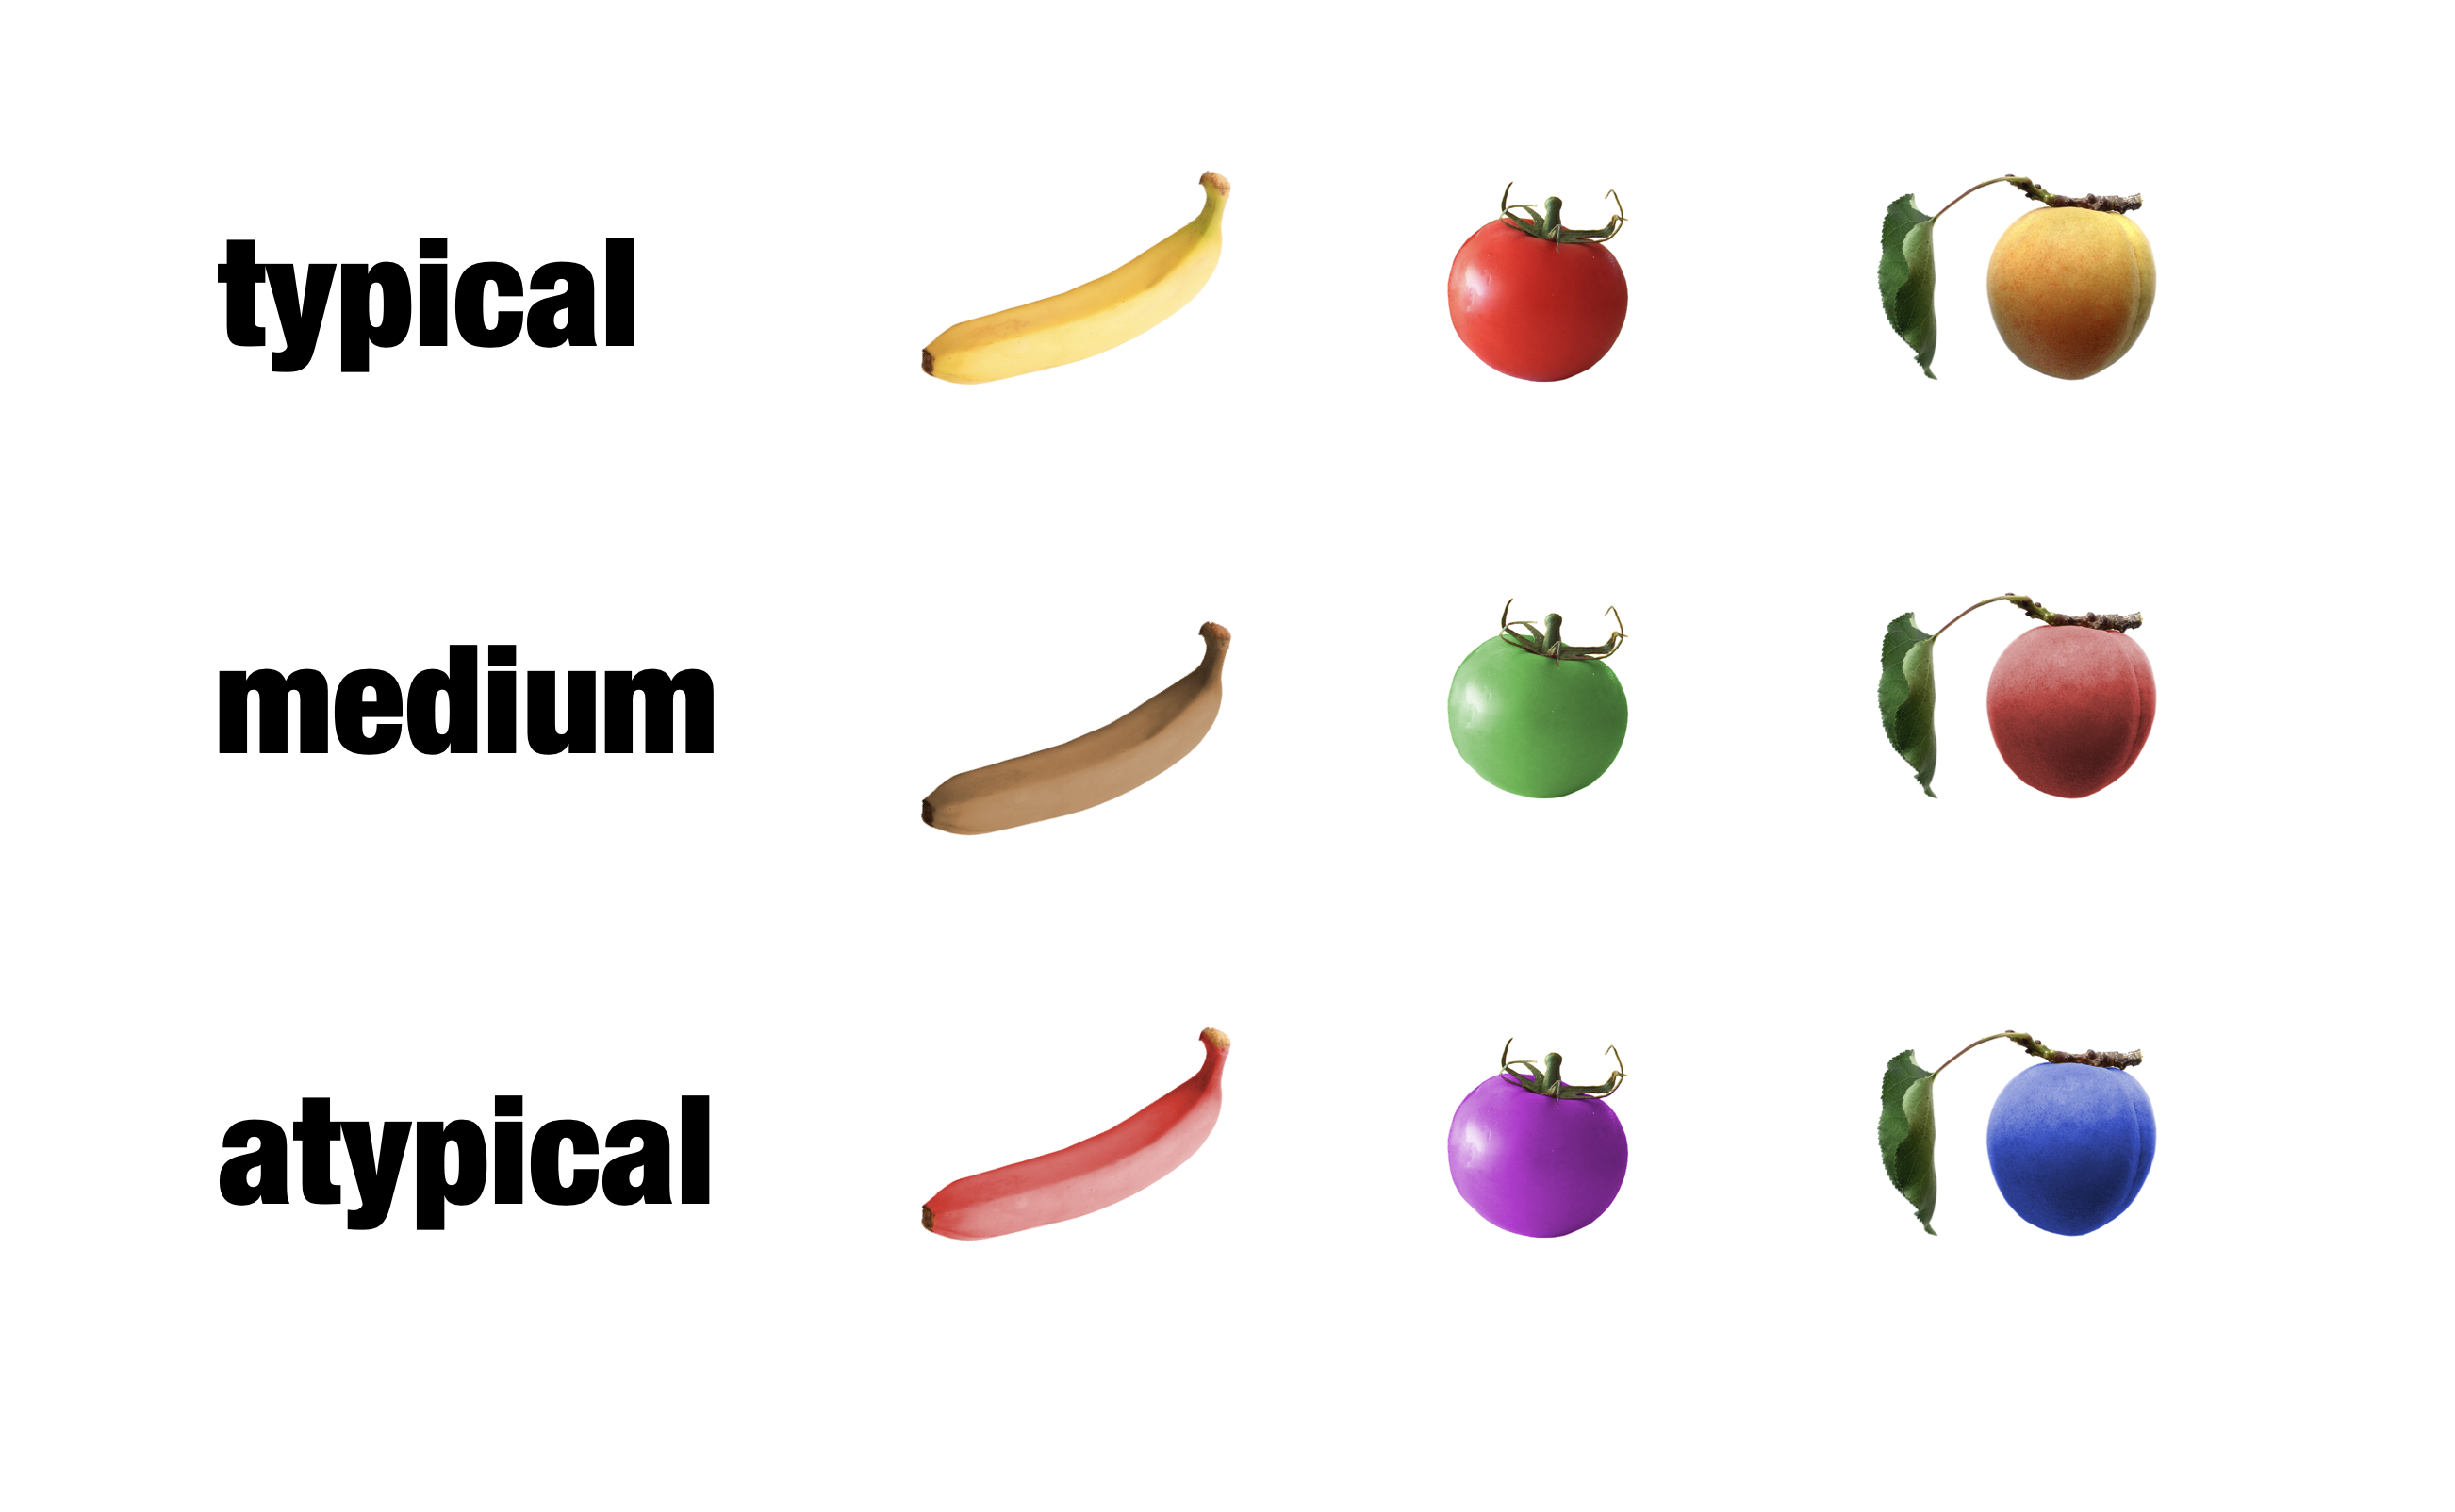
\includegraphics[width=0.6\linewidth]{typicality_examples} 

}

\caption{Three examples for typical, medium typical and atypical combinations of colour and object.}\label{fig:image0}
\end{figure}

Participants were seated in front of a computer screen. The experimenter
sat at the opposite side of the table in front of another computer
screen. The participants and the experimenter could see neither each
other nor each others' screens. The experiment consisted of two phases:
a familiarization phase and a test phase.

In a familiarization phase, participants saw one object per trial. In
order to advance to the next trial, participants had to read out loud
the corresponding noun phrase (e.g.~blue banana). During this phase,
participants had to name all atypical colour-object targets that we used
in the test phase of the experiment alongside their typical
counterparts. For example, if red banana (atypical) was an experimental
target, participants were presented with both the red banana (atypical)
and the yellow banana (typical). This familiarization phase was included
in order to ensure that participants can relate typical and atypical
colour-object combinations to each other.

After the familiarization phase, participants entered the test phase. On
each trial in the test phase, participants first saw four coloured
objects in the top left, top right, bottom left, and bottom right of the
screen, respectively. One of the object served as the target; another
served as the competitor; and the remaining two served as unrelated
distractors. The position of the visual stimuli was randomized for each
trial and each participant. In the center of the screen, a black cube
was displayed which could be moved by the experimenter. The participants
were asked to instruct the experimenter to move the cube onto one of the
four pictures.

Each test trial consisted of two parts. The `trigger' instruction and
the `test' instruction. After the preview of all images was displayed
for 1500 ms, the competitor object was visually highlighted by an arrow,
and a `trigger' instruction was orthographically presented below the
cube (see Figure \#):

\ex \begingl
\glpreamble Du sollst den Würfel auf der grünen Sonnenbrille ablegen.//
\gla du sollst den würfel auf der grünen sonnenbrille ablegen.//
\glb you have.to the cube on the green sunglasses put//
\glft `You have to put the cube on top of the green sunglasses.'//
\endgl \xe

\begin{figure}[tbp]

{\centering 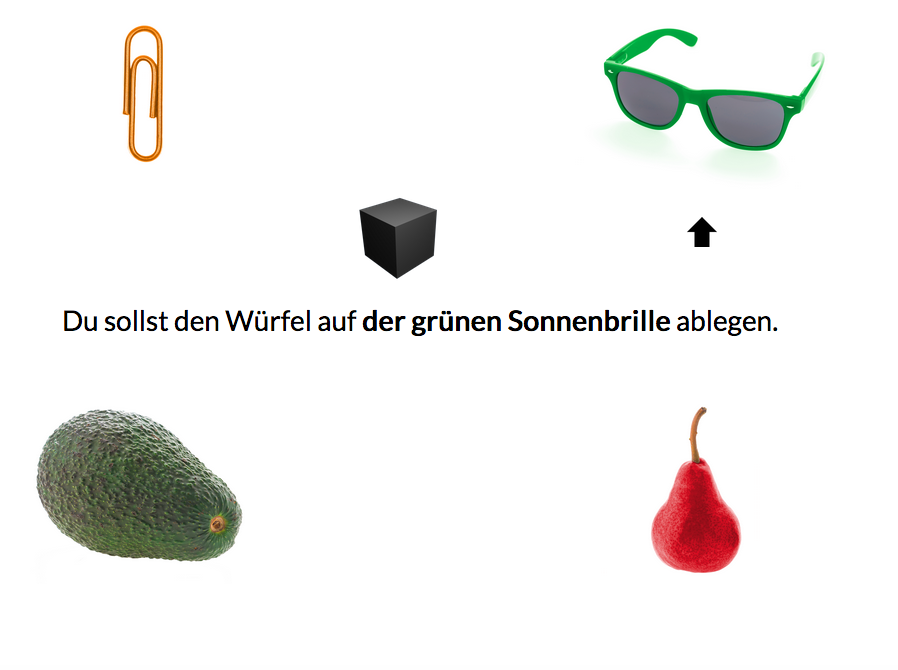
\includegraphics[width=0.6\linewidth]{sample_experiment_screen_competitor} 

}

\caption{Example screen at the beginning of a trials. The discourse setting trigger sentence is displayed in the middle below the cube. The participants have to instruct the experimenter to move the cube on top of the green sunglasses (indicated by an arrow).}\label{fig:image1}
\end{figure}

The trigger instruction was supposed to create a discourse context, such
that both the color and the competitor object were introduced as
background information into the discourse (here: green and sunglasses).
The trial proceeded when the experimenter has moved the cube onto the
respective referent. The sentence and the arrow disappeared.
Subsequently, the target object was visually highlighted by an arrow and
the test instruction was presented containing the target object (see
Figure \#):

\ex \begingl
\glpreamble Und jetzt sollst du den Würfel auf der grünen Avokado ablegen.//
\gla und jetzt sollst du den würfel auf der grünen avokado ablegen//
\glb and now have.to you the cube on the green avocado put//
\glft `And now, you have to put the cube on top of the green avocado.'//
\endgl \xe

\begin{figure}[tbp]

{\centering 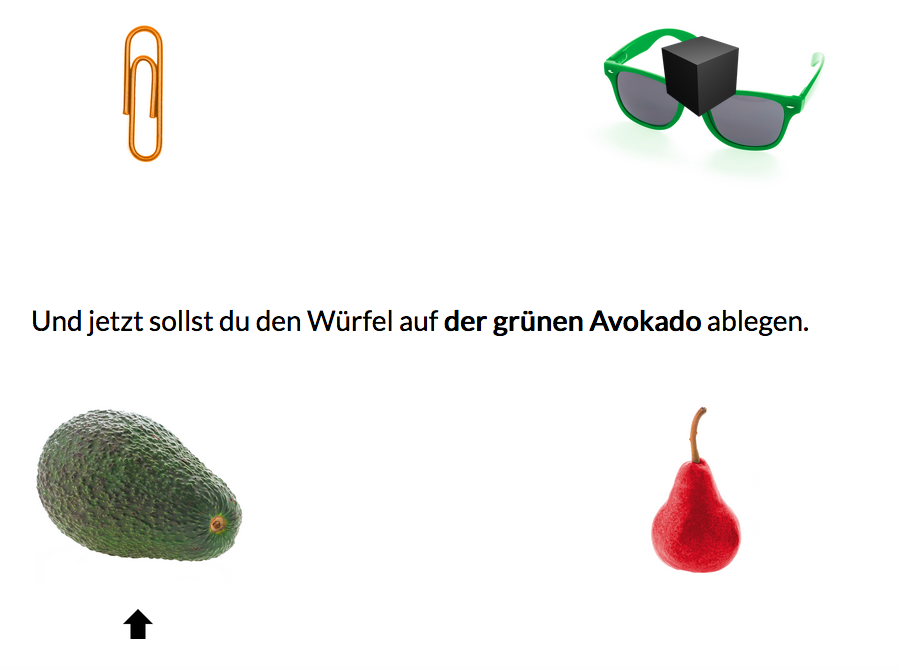
\includegraphics[width=0.6\linewidth]{sample_experiment_screen_target} 

}

\caption{Example screen after the trigger sentence. The target sentence is displayed in the middle of the screen. Now, participants have to instruct the experimenter to move the cube on top of the green avocado (indicated by an arrow).}\label{fig:image2}
\end{figure}

The trial was completed and the next trial initiated as soon as the
experimenter had moved the cube to the target referent. There was a 3000
ms inter stimulus interval between trials (grey screen). In both
competitor and target sub sequences, the arrow was displayed with a lag
of 1000 ms and the target sentence with a lag of 1500 ms in order to
give participants sufficient time to glance at all referents before they
were able to identify the relevant object and the instructions.

Using the trigger instruction to set up the discourse context enabled us
to manipulate the focus structure of the target sentence. If the color
of the competitor and the target are of the same object type but
differed in color (e.g.~yellow banana --\textgreater{} blue banana), the
color adjective was discourse-pragmatically focused (henceforth the
Adjective Focus (AF) condition). If the objects differed but not their
color (e.g.~yellow banana --\textgreater{} yellow tomato), the noun was
in focus (henceforth the Noun Focus (NF) condition). If both the color
and the object differed (e.g.~yellow banana --\textgreater{} blue
tomato), the whole noun phrase was in focus (henceforth the Double Focus
(DF) condition).

We are interested in the Noun Focus condition, only. AF and DF served as
filler trials. There were 15 NF trials, 10 AF and 10 DF trials each.
Each trial occurred two times per participants, yielding a total of 70
trials per participant.

The experimental program (implemented as a browser-based application) is
available here: \url{https://github.com/SBRitter/fruits-production}.

\appendix

\hypertarget{adds}{%
\section{Additional Information}\label{adds}}

Here we specify in detail, how stimuli were selected for the above
described production study.

\hypertarget{selection-of-stimuli-superset}{%
\subsection{Selection of stimuli
superset}\label{selection-of-stimuli-superset}}

The selection of stimuli was informed by a norming study for which we
selected twenty fruits or vegetables (henceforth: FOODs) and four other
referents (henceforth: NON-FOODs). Selection criteria were mainly
informed by visual discriminability and phonemic composition, such that
nouns denoting our objects were supposed to contain few voiceless
segments.

For each of the FOODs and NON-FOODs, we created colored versions by
image manipulation using \href{http://www.gimp.org}{gimp}. Images of all
individual objects were collected from internet databases containing
copyright-free high-resolution images
(e.g.~\href{https://pixabay.com}{Pixabay}). During the manipulation
process, the background of the pictures was replaced by a white
background. In order to change the color of the objects, a layer in the
respective color was created and overlaid on top of the original image
using ``Color'' as the layer mode. The hexadecimal color codes for the
colors that we used are listed below:

\noindent Blue: \#29429f\\
\noindent Green: \#3f8535\\
\noindent Red: \#9d1c1c\\
\noindent Purple: \#6d1b79\\
\noindent Brown: \#2a1d11\\
\noindent Yellow: \#e3c917\\
\noindent Orange: \#ff8400\\
\noindent Orange (potatoes): \#ff6600\\
\noindent Black: \#000000\\
\noindent Grey: \#FFFFFF

All pictures with natural and manipulated colors are available here:
\url{https://osf.io/rdtx5/}.

The colors for the twenty FOODs were subjectively selected to reflect a
range of compatibilities with the respective objects, e.g.~a typical
banana is yellow; a less typical banana could be brown (too ripe) or
green (not yet ripe); and an atypical banana could be blue. Every FOOD
was presented in four of nine manipulated colors alongside its original
image. The four NON-FOODs were subjectively selected to represent color
agnostic objects which can and do come in a variety of colors. All
objects were chosen such that their respective German nouns were either
feminine singular (e.g.~``die Banana'' `the banana') or plural
(e.g.~``die Trauben'' `the grapes').

We used the following FOODs: apricot, avocado, banana, beans, carrot,
cherry, cucumber, eggplant, grapes, lemon, mandarine, pear, pepper,
pineapple, potatoes, strawberry, tomato, walnut, zucchini.

We used the following NON-FOODs: clothespin, paper clip, socks,
sunglasses.

\hypertarget{the-norming-study}{%
\subsection{The norming study}\label{the-norming-study}}

One-hundred German native speakers participated in a norming study using
the crowd sourcing platform
{[}Prolific{]}{]}(\url{https://www.prolific.ac}). We presented all
objects in different colors to our participants. FOODs came in 5 colors
per object, NON-FOODs came in all nine colors. Participants were
instructed to rate how typical they think the color for each object was,
using a smooth slider ranging from 1 to 100 (see javascript for the
experimental design here:
\url{https://github.com/stelaseldano/colour-typicality-norming}. The
results of the norming study can be retrieved here:
\url{https://osf.io/znpg5/}.

\hypertarget{selection-of-experimental-stimuli}{%
\subsection{Selection of experimental
stimuli}\label{selection-of-experimental-stimuli}}

The norming ratings were subsequently used to select appropriate stimuli
for the production study according to the following procedure:

First, we chose five colors from the norming data set: yellow, green,
red, orange, and brown. Those were the most frequent colors in the
superset and their norming results varied strongly as a function of the
object.

Second, we sorted the FOODs according to their typicality ratings and
binned them into typical, medium, and atypical. Typical FOODs were
defined by norming ratings above 90. Atypical FOODs were defined by
norming ratings below 25. Medium typical FOODs were defined by norming
ratings in between 25 and 90. For each color and typicality, we selected
one FOOD object. Each cell was occupied by a different FOOD.

For the critical focus condition (NF) this selection procedure resulted
in 15 target FOODs (5 colors x 3 typicality categories):

\noindent atypical:\\
\noindent Yellow cherry (Gelbe Kirsche)\\
\noindent Green carrot (Grüne Möhre)\\
\noindent Red cucumber (Rote Gurke)\\
\noindent Orange grapes (Oangene Trauben)\\
\noindent Brown pepper (Braune Paprika)

\noindent medium:\\
\noindent Yellow peas (Gelbe Erbsen)\\
\noindent Green tomato (Grüne Tomate)\\
\noindent Red apricot (Rote Aprikose)\\
\noindent Orange potatoes (Orangene Kartoffeln)\\
\noindent Brown banana (Braune Banane)

\noindent typical:\\
\noindent Yellow lemon (Gelbe Zitrone)\\
\noindent Green green beans (Grüne Bohnen)\\
\noindent Red strawberry (Rote Erdbeere)\\
\noindent Orange mandarine (Orangene Mandarine)\\
\noindent Brown walnut (Braune Walnuss)

The set of 15 competitors from the NON-FOOD subset was selected to
ensure that there are as many distinct competitors for each color as
there are target objects. The set consisted of the following objects:

\noindent Yellow sunglasses (Gelbe Sonnenbrille)\\
\noindent Yellow socks (Gelbe Socken)\\
\noindent Yellow clothes peg (Gelbe Wäscheklammer)\\
\noindent Green sunglasses (Grüne Sonnenbrille)\\
\noindent Green socks (Grüne Socken)\\
\noindent Green Paper clip (Grüne Büroklammer)\\
\noindent Red socks (Rote Socken)\\
\noindent Red paper clip (Rote Büroklammer)\\
\noindent Red clothes peg (Rote Wäscheklammer)\\
\noindent Orange socks (Orangene Socken)\\
\noindent Orange paper clip (Orangene Büroklammer)\\
\noindent Orange clothes peg (Orangene Wäscheklammer)\\
\noindent Brown sunglasses (Braune Sonnenbrille)\\
\noindent Brown paper clip (Braune Büroklammer)\\
\noindent Brown clothes peg (Braune Wäscheklammer)

The pairing of targets and competitors was randomized for each subject,
with the only constraint that the competitor had the same color as the
target object (e.g.~if blue banana was the target, blue grapes is a
possible competitor) (see randomization section below for more details).

For the filler focus conditions (AF + DF), we distributed FOODs and
NON-FOODs to fulfil the following constraints: (a) each target FOOD
appeared 3 times and (b) each color appeared as a traget color 14 times.

For all three focus conditions, a subset of distractors was selected
from the initial superset: Distractors were either FOODS that were
neither used as targets nor as competitors (avocado, egg plant, pear,
zucchini) or NON-FOODs. Within each given trial, the distractors did
neither share color nor object identity with neither the target nor the
competitor.

Overall, the sets of target, competitors and distractors are combined
such that all five colors occurred equally often throughout the
experiment (= 28 times).

\hypertarget{randomization}{%
\section{Randomization}\label{randomization}}

For each trial, targets, competitors, and distractors are chosen in a
randomized way, fulfilling the following requirements:

\begin{itemize}
\item
  NF-Condition:\\
  Color of Target = Color of Competitor\\
  Object of Target != Object of Competitor
\item
  AF-Condition:\\
  Color of Target != Color of Competitor\\
  Object of Target = Object of Competitor
\item
  DF-Condition:\\
  Color of Target != Color of Competitor\\
  Object of Target != Object of Competitor
\item
  All conditions:\\
  Both distractors have to differ in color and object identity from both
  target and competitor.
\end{itemize}

The competitor and distractors are matched iteratively to a target. One
competitor could only be used twice or a third time if all other
competitors that were left had been considered and prove inappropriate.

The set of four objects (quadruple) was formed separately for each
condition. After the three lists had been compiled, they were merged.
The sequence of quadruples was randomized such that the following
requirements were met:

\begin{itemize}
\tightlist
\item
  The target color of one quadruple must not be equal to the competitor
  color of the following quadruple in order to avoid a contrastive focus
  on the next competitor noun.
\item
  The target object of one quadruple must not be equal to the competitor
  object of the following quadruple to avoid a contrastive focus on the
  next competitor adjective.
\item
  The list can have the same experimental condition in adjacent trials
  only in maximally 12\% of all cases.
\end{itemize}

Following these criteria, one randomized list for each subject was
produced. The list was then copied and merged with the first list in
order to ensure that each unique trial occurs twice during one recording
session. In case the copy-and-merge procedure led to violation of any of
the criteria described above, the first trial of the repetition list was
shuffled until the criteria were met.

The python code for the randomization is available here:
\url{https://github.com/SBRitter/fruits-randomization}.

\end{document}
